\section{Results}

\subsection{Quality evaluation}

The RNA-seq data was initially assessed with FastQC\index{FastQC}, and according to this assessment the data was preprocessed/trimmed with Trimmomatic\index{Trimmomatic} and afterwards assessed again with FastQC. Finally, an overall report on the data preprocessing, the quality assessments and the kallisto\index{kallisto} pseudoalignments was created with MultiQC\index{MultiQC}.

Figure \ref{fig:0.1-MultiQC_FastQC_status_checks} shows the MultiQC report on the Trimmomatic\index{Trimmomatic} preprocessing (the surviving reads).

\begin{figure}[htbp]
    \caption{Trimmomatic preprocessing}
    \label{fig:0.1-MultiQC_FastQC_status_checks}
    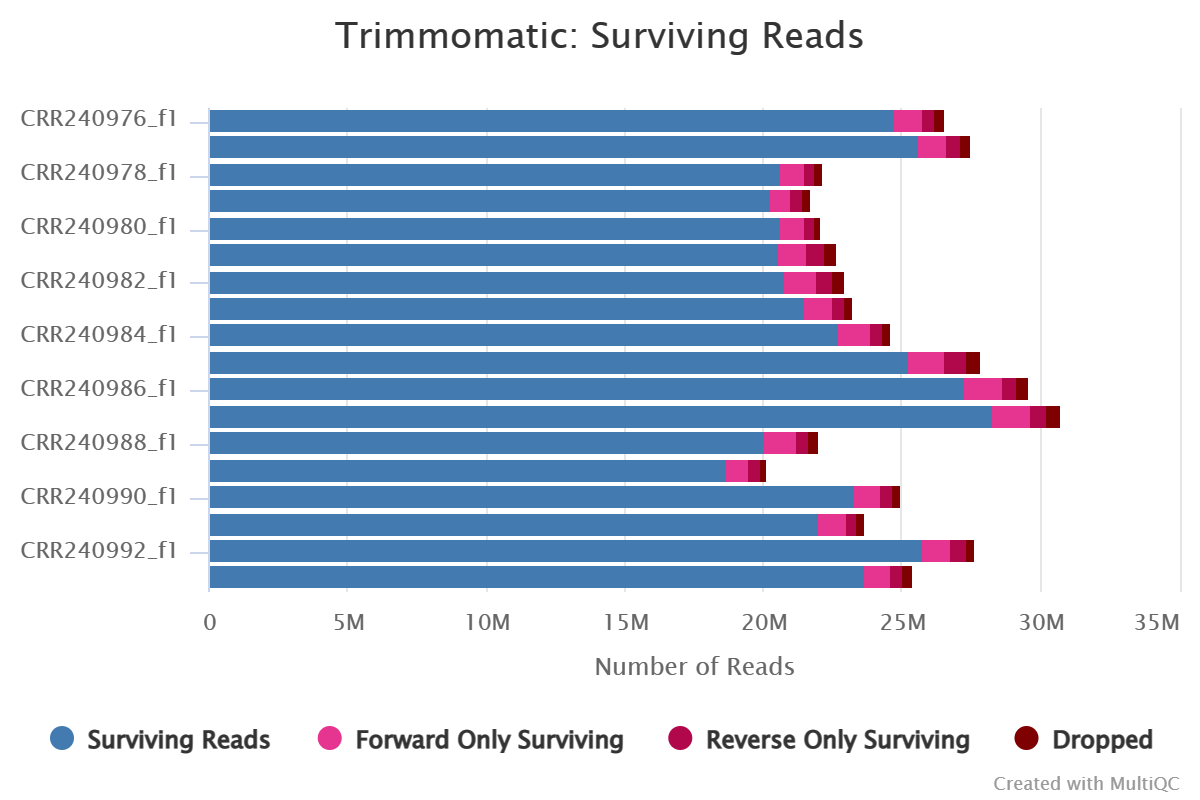
\includegraphics[width=0.75\textwidth]{../../results/multiqc/Plot-Exports/trimmomatic-surviving_reads}
\end{figure}

Figure \ref{fig:0.2-MultiQC_FastQC_status_checks} shows the MultiQC overview of the FastQC\index{FastQC} quality assessments of the trimmed FASTQ files.

\begin{figure}[htbp]
    \caption{FastQC quality assessment of the preprocessed FASTQ files}
    \label{fig:0.2-MultiQC_FastQC_status_checks}
    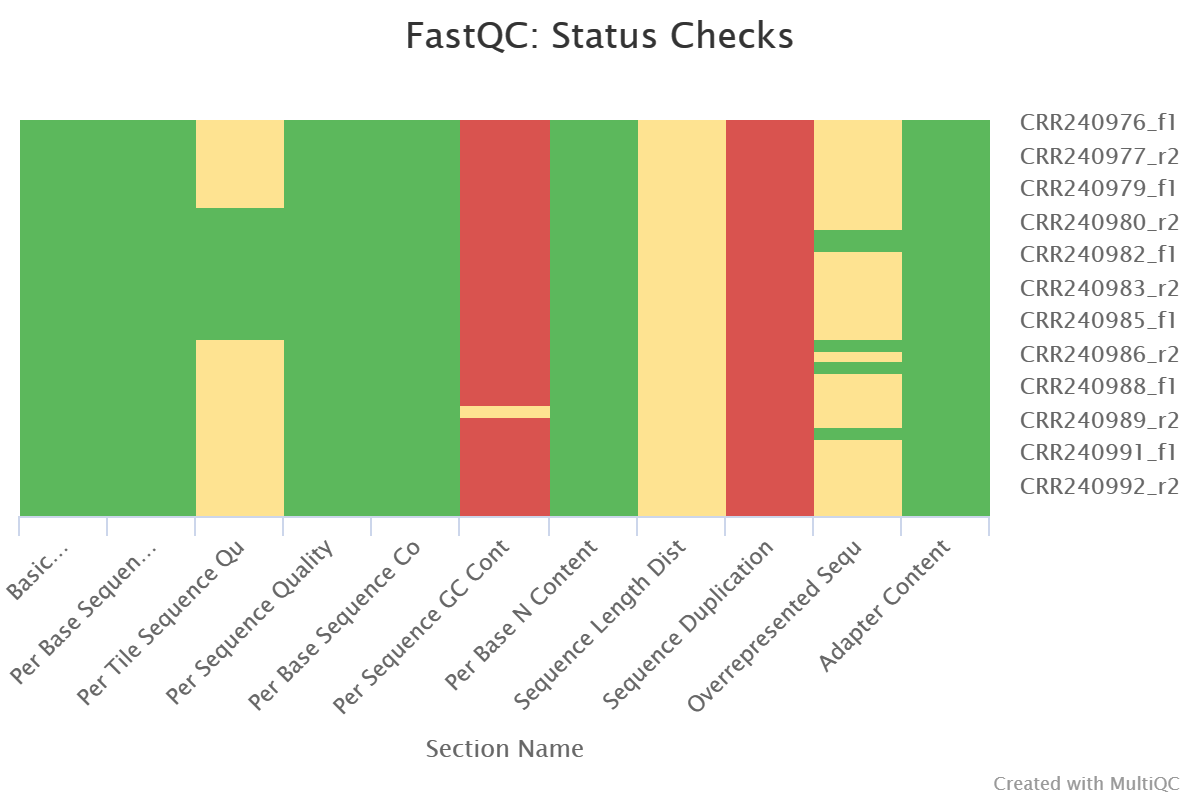
\includegraphics[width=0.75\textwidth]{../../results/multiqc/Plot-Exports/fastqc-status-check-heatmap}
\end{figure}

According to these quality assessments, the (trimmed) RNA-seq data may be regarded as good quality for the purpose of this research.


\subsection{Reads mapped to the reference transcriptome}

For most of the FASTQ files, kallisto pseudoaligned well above 80 \% of the (preprocessed) RNA-seq reads. Figure \ref{fig:0.3-MultiQC_kallisto_alignment} shows a MultiQC overview of the kallisto\index{kallisto} pseudoalignments.

\begin{figure}[htbp]
    \caption{kallisto pseudoalignments}
    \label{fig:0.3-MultiQC_kallisto_alignment}
    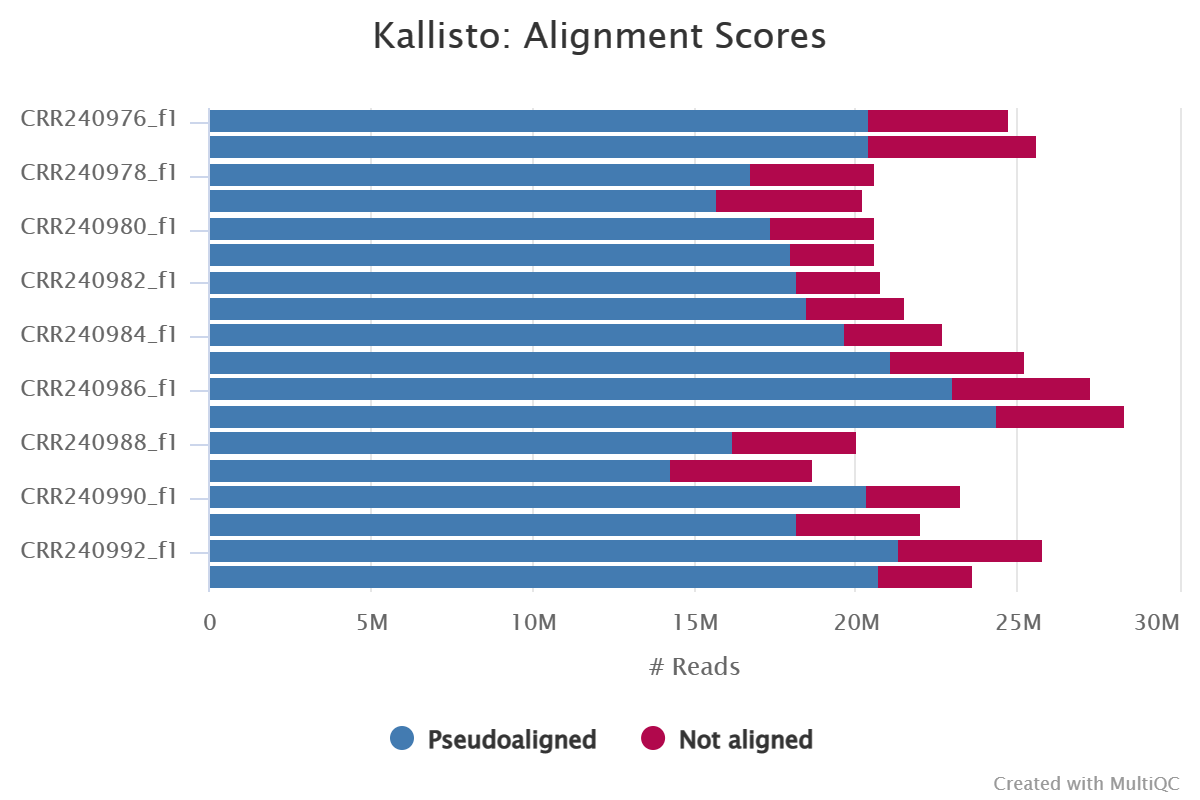
\includegraphics[width=0.75\textwidth]{../../results/multiqc/Plot-Exports/kallisto_alignment}
\end{figure}


\subsection{Hierarchical cluster analysis}

The hierarchical cluster analysis\index{hierarchical cluster analysis (HCA)} reveals that the normal condition groups and the drought stress condition groups are closely related (grouped together). But the data for O. nivara also shows that the cultivar has an even greater impact on the clustering then the drought stress condition (see figures \ref{fig:3.1-Clust-Dendrogram-Oryza_nivara} and \ref{fig:3.1-Clust-Dendrogram-Oryza_sativa}).

\begin{figure}[htbp]
    \caption{Hierarchical cluster analysis of the O. nivara RNA-seq data}
    \label{fig:3.1-Clust-Dendrogram-Oryza_nivara}
    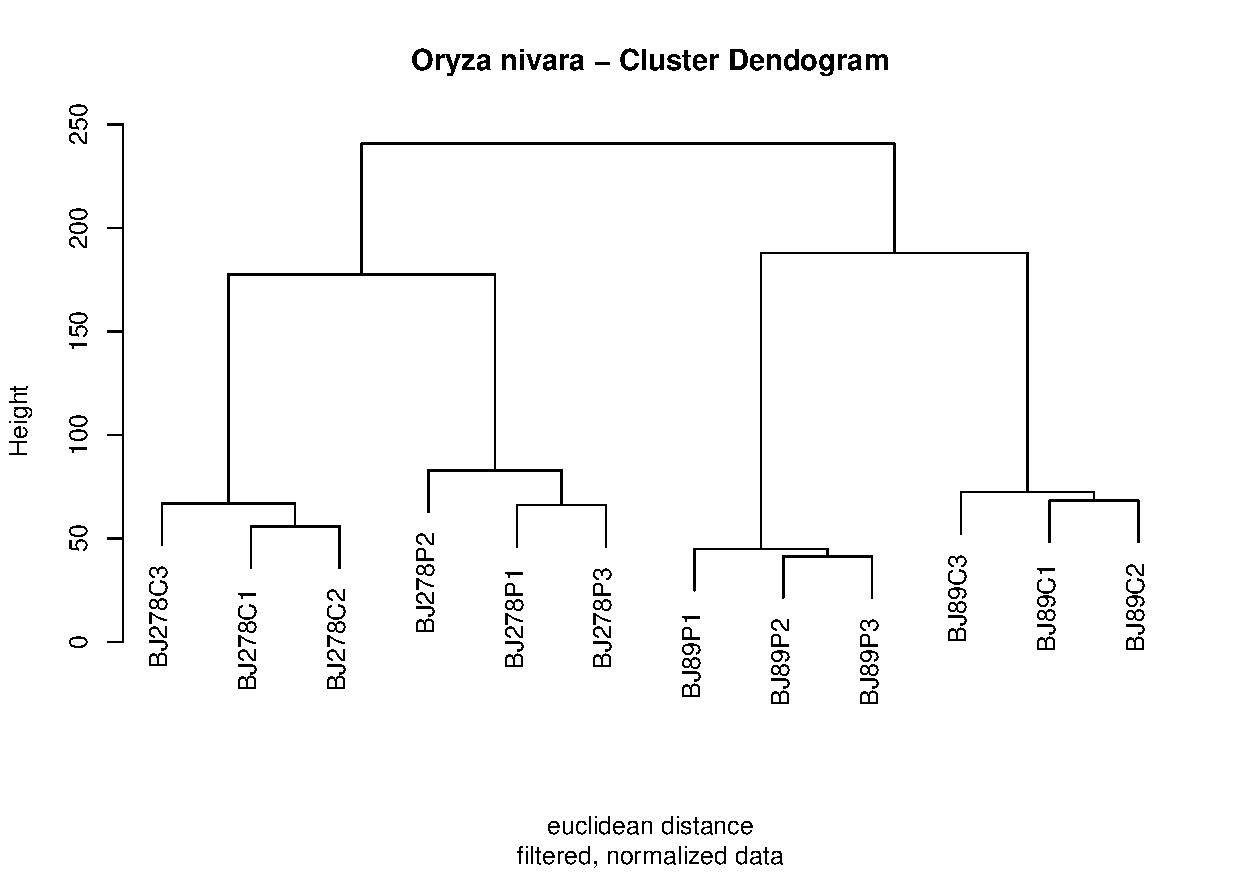
\includegraphics[width=0.75\textwidth]{../../results/plots-and-tables/3.1-Clust-Dendrogram-Oryza_nivara}
\end{figure}

\begin{figure}[htbp]
    \caption{Hierarchical cluster analysis of the O. sativa RNA-seq data}
    \label{fig:3.1-Clust-Dendrogram-Oryza_sativa}
    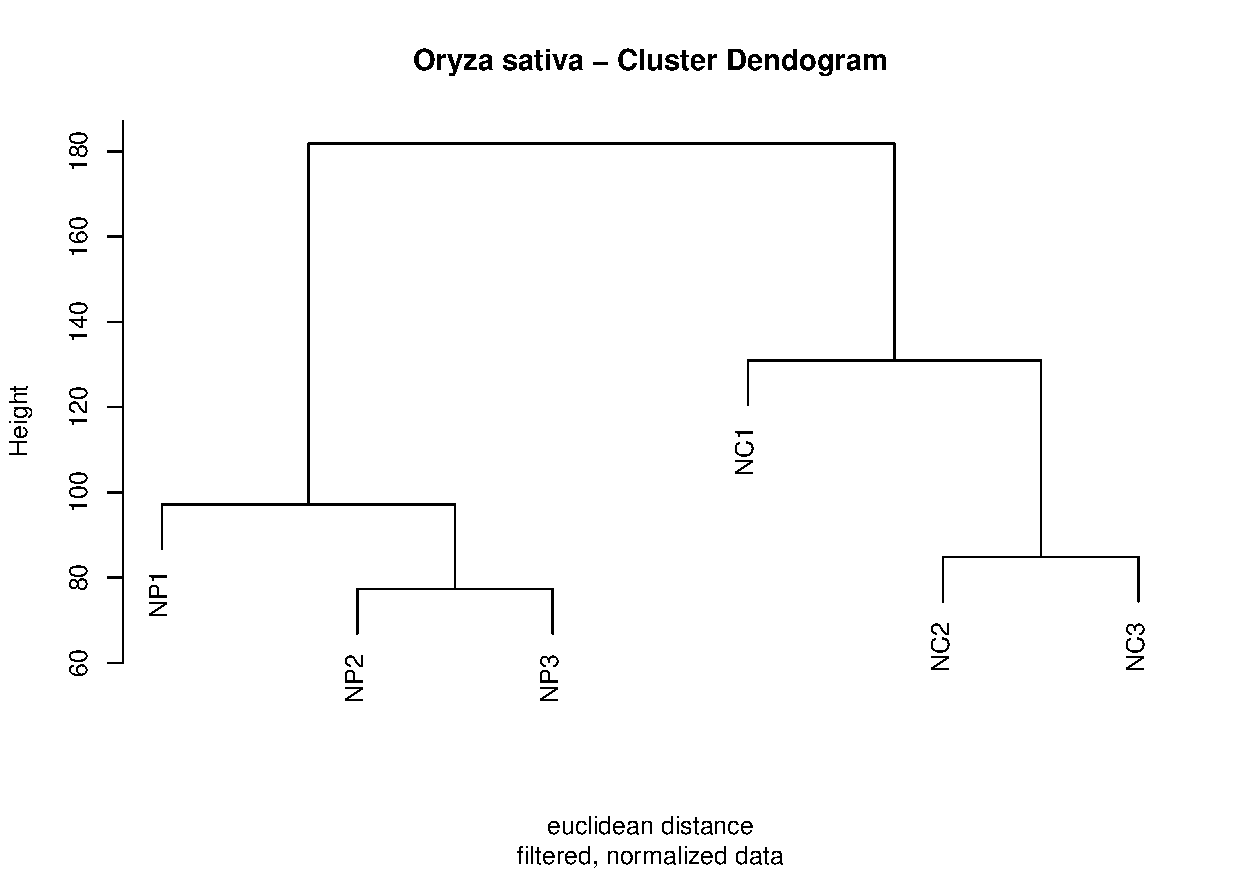
\includegraphics[width=0.75\textwidth]{../../results/plots-and-tables/3.1-Clust-Dendrogram-Oryza_sativa}
\end{figure}


\subsection{Principal component analysis}

The principal component analysis (PCA)\index{principal component analysis (PCA)} reveals that for both O. nivara and O. sativa the first two principal components account for more than 80 \% of the variance in the gene expression. Figures  \ref{fig:3.2-PCA-Oryza_nivara} and \ref{fig:3.2-PCA-Oryza_sativa} show the contribution percentage of the samples to the first two principal components (PCs)\index{principal component analysis (PCA)!principal component (PC)} for the two species.

For O. nivara, the samples from the same condition (normal vs drought stress) cluster together, with a tight clustering of the two different cultivars. This means that the different conditions might well explain the differences in gene expression, with the cultivar being an important confounding factor.

For O. sativa, the samples from the same condition cluster together with the exception of sample "NC1". This might be due to a batch effect\index{batch effect}.

\begin{figure}[htbp]
    \caption{PCA of the log2(CPM) data - O. nivara}
    \label{fig:3.2-PCA-Oryza_nivara}
    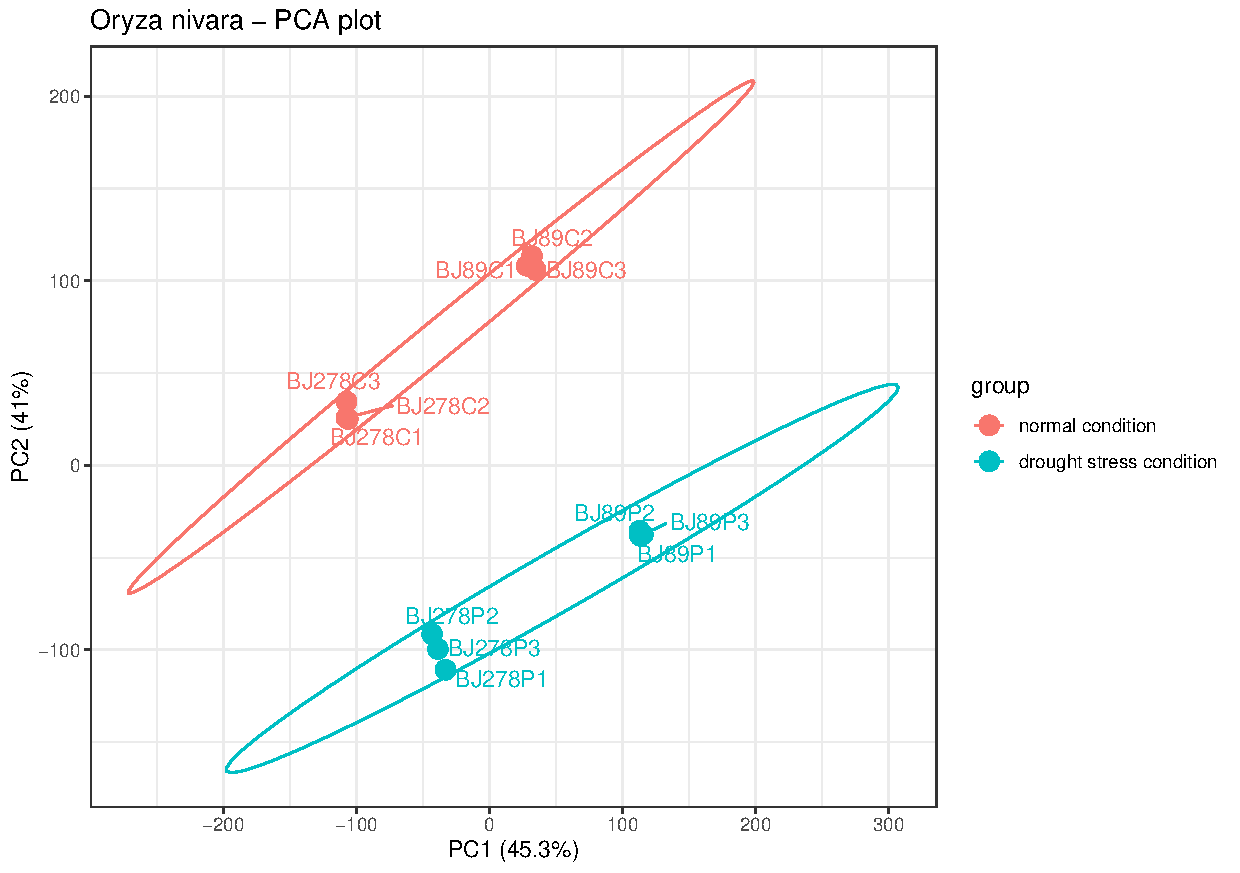
\includegraphics[width=0.9\textwidth]{../../results/plots-and-tables/3.2-PCA-Oryza_nivara}
\end{figure}

\begin{figure}[htbp]
    \caption{PCA of the log2(CPM) data - O. sativa}
    \label{fig:3.2-PCA-Oryza_sativa}
    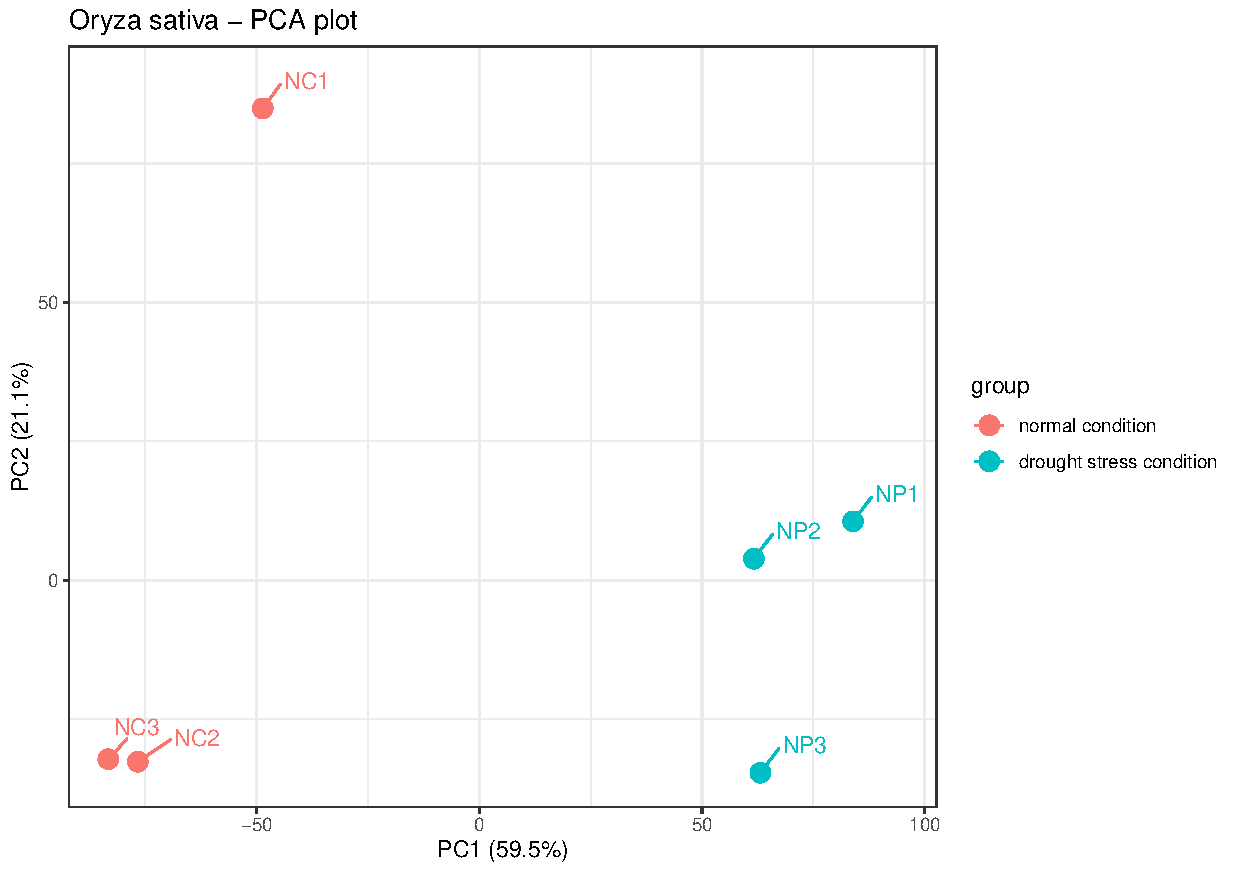
\includegraphics[width=0.9\textwidth]{../../results/plots-and-tables/3.2-PCA-Oryza_sativa}
\end{figure}


\subsection{Differentially expressed genes}

The volcano plots \ref{fig:4.1-DEG-Volcano-Plot-Oryza_nivara} and \ref{fig:4.1-DEG-Volcano-Plot-Oryza_sativa} provide a quick overview of the genes with large fold changes that are also statistically significant. These may be the biologically most significant genes.

\begin{figure}[htbp]
    \caption{Volcano plot of the DEGs - O. nivara}
    \label{fig:4.1-DEG-Volcano-Plot-Oryza_nivara}
    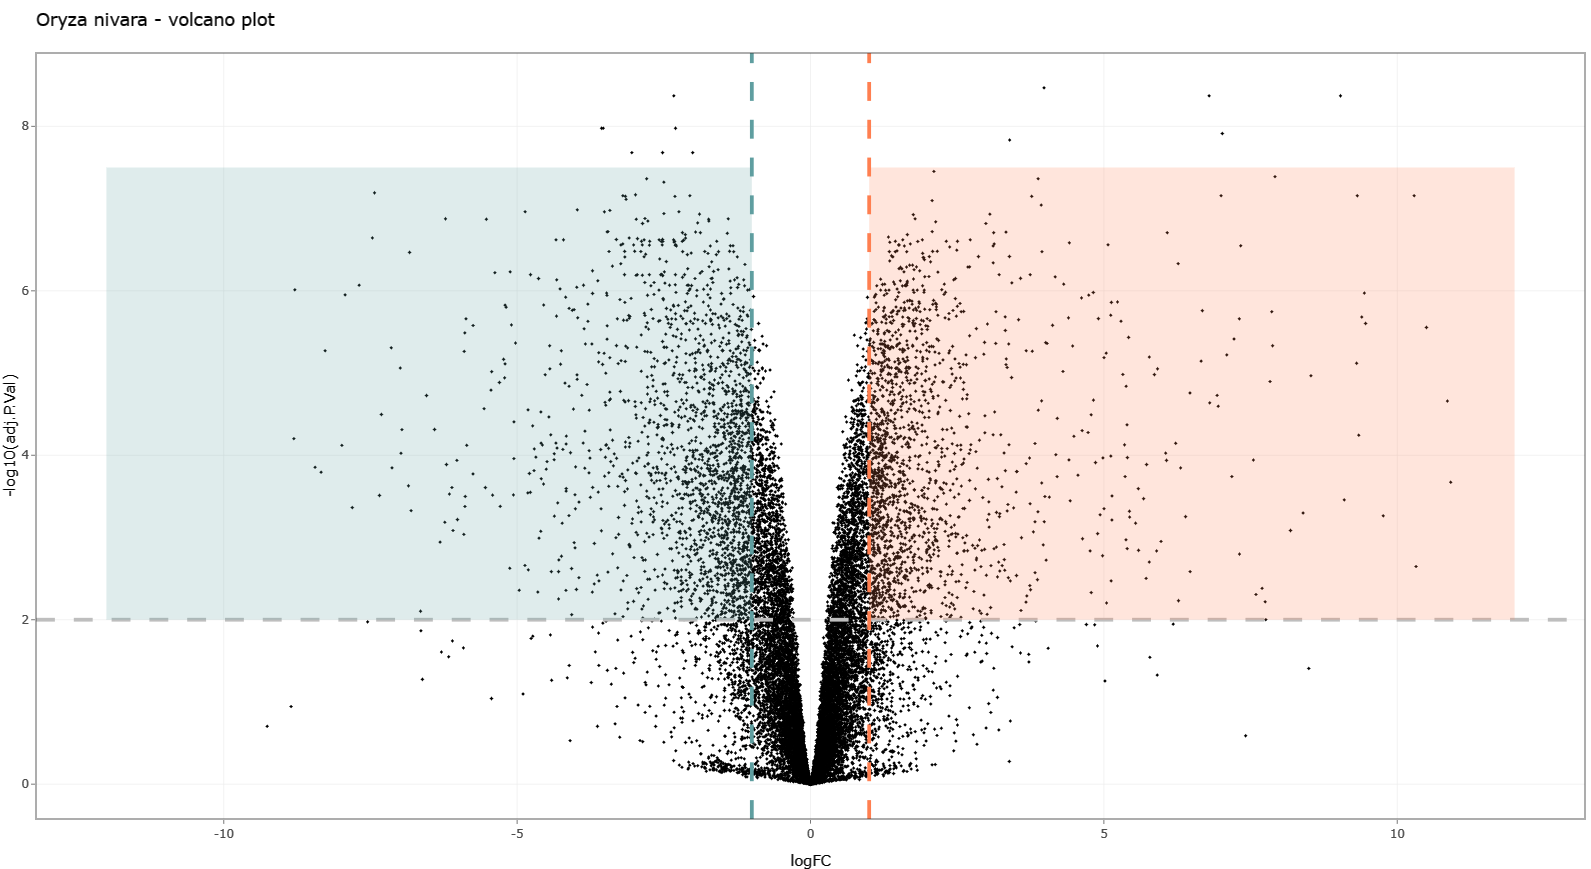
\includegraphics[width=0.9\textwidth]{../../results/plots-and-tables/4.1-DEG-Volcano-Plot-Oryza_nivara}
\end{figure}

\begin{figure}[htbp]
    \caption{Volcano plot of the DEGs - O. sativa}
    \label{fig:4.1-DEG-Volcano-Plot-Oryza_sativa}
    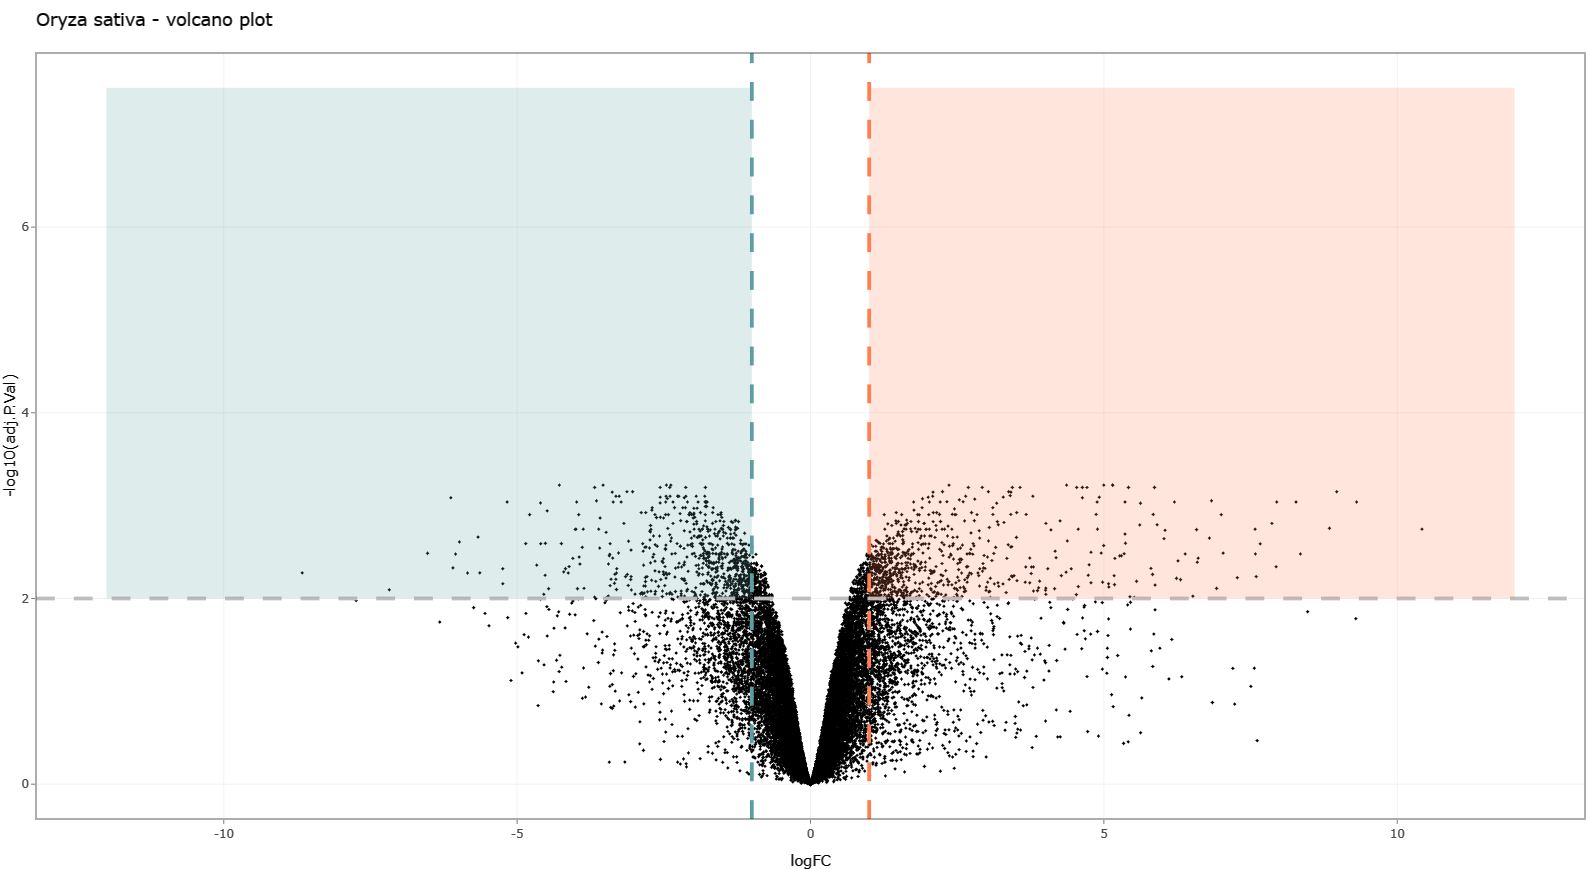
\includegraphics[width=0.9\textwidth]{../../results/plots-and-tables/4.1-DEG-Volcano-Plot-Oryza_sativa}
\end{figure}

According to the limma tests with a p-value of one percent, there are 15 down- vs 33 up-regulated genes for O. nivara under drought stress conditions, and 2 down- vs 16 up-regulated for O. sativa. Figure \ref{fig:4.2-DEG-Venn-Diagr} shows the respective Venn diagrams. Figures \ref{fig:4.4-DEG-Heatmap-Oryza_nivara} and \ref{fig:4.4-DEG-Heatmap-Oryza_sativa} present heatmaps of these genes.

\begin{figure}[htbp]
    \caption{Venn diagrams of the DEGs}
    \label{fig:4.2-DEG-Venn-Diagr}
    \begin{subfigure}[t]{0.44\linewidth}
        \caption{O. nivara}
        \label{fig:4.2-DEG-Venn-Diagr-Oryza_nivara}
        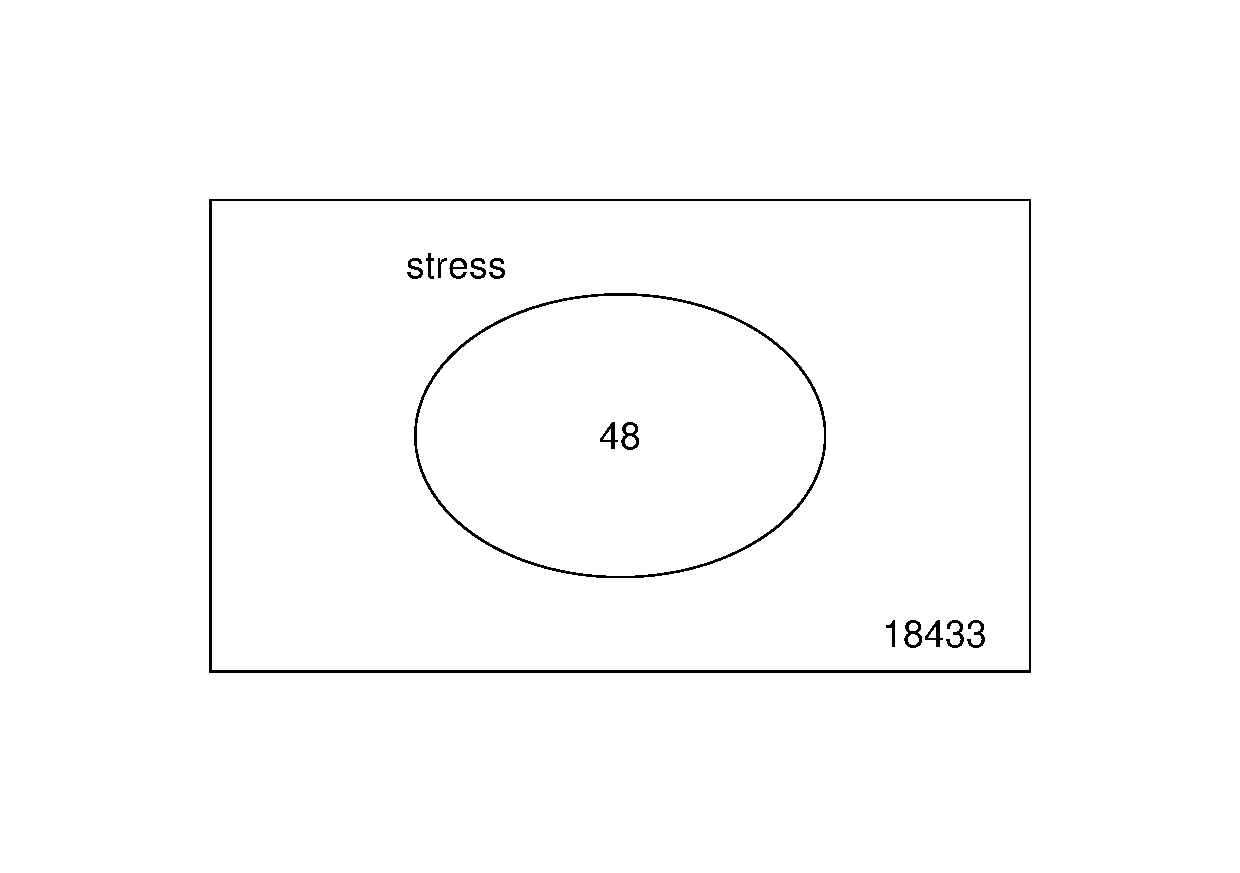
\includegraphics[width=\textwidth, height=4cm]{../../results/plots-and-tables/4.2-DEG-Venn-Diagr-Oryza_nivara}
    \end{subfigure}
    \begin{subfigure}[t]{0.44\linewidth}
        \caption{O. sativa}
        \label{fig:4.2-DEG-Venn-Diagr-Oryza_sativa}
        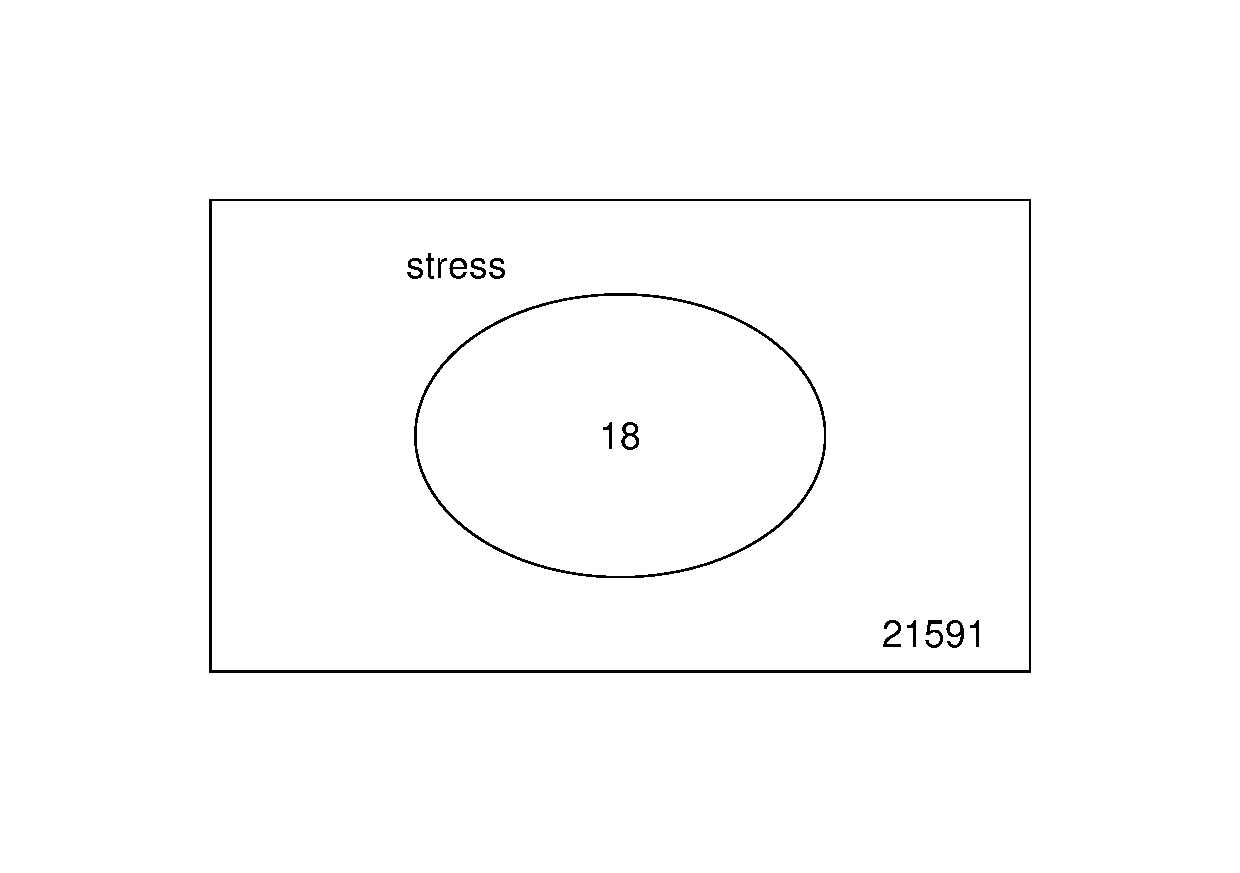
\includegraphics[width=\textwidth, height=4cm]{../../results/plots-and-tables/4.2-DEG-Venn-Diagr-Oryza_sativa}
    \end{subfigure}
\end{figure}

\begin{figure}[htbp]
    \caption{Heatmap of the DEGs - O. nivara}
    \label{fig:4.4-DEG-Heatmap-Oryza_nivara}
    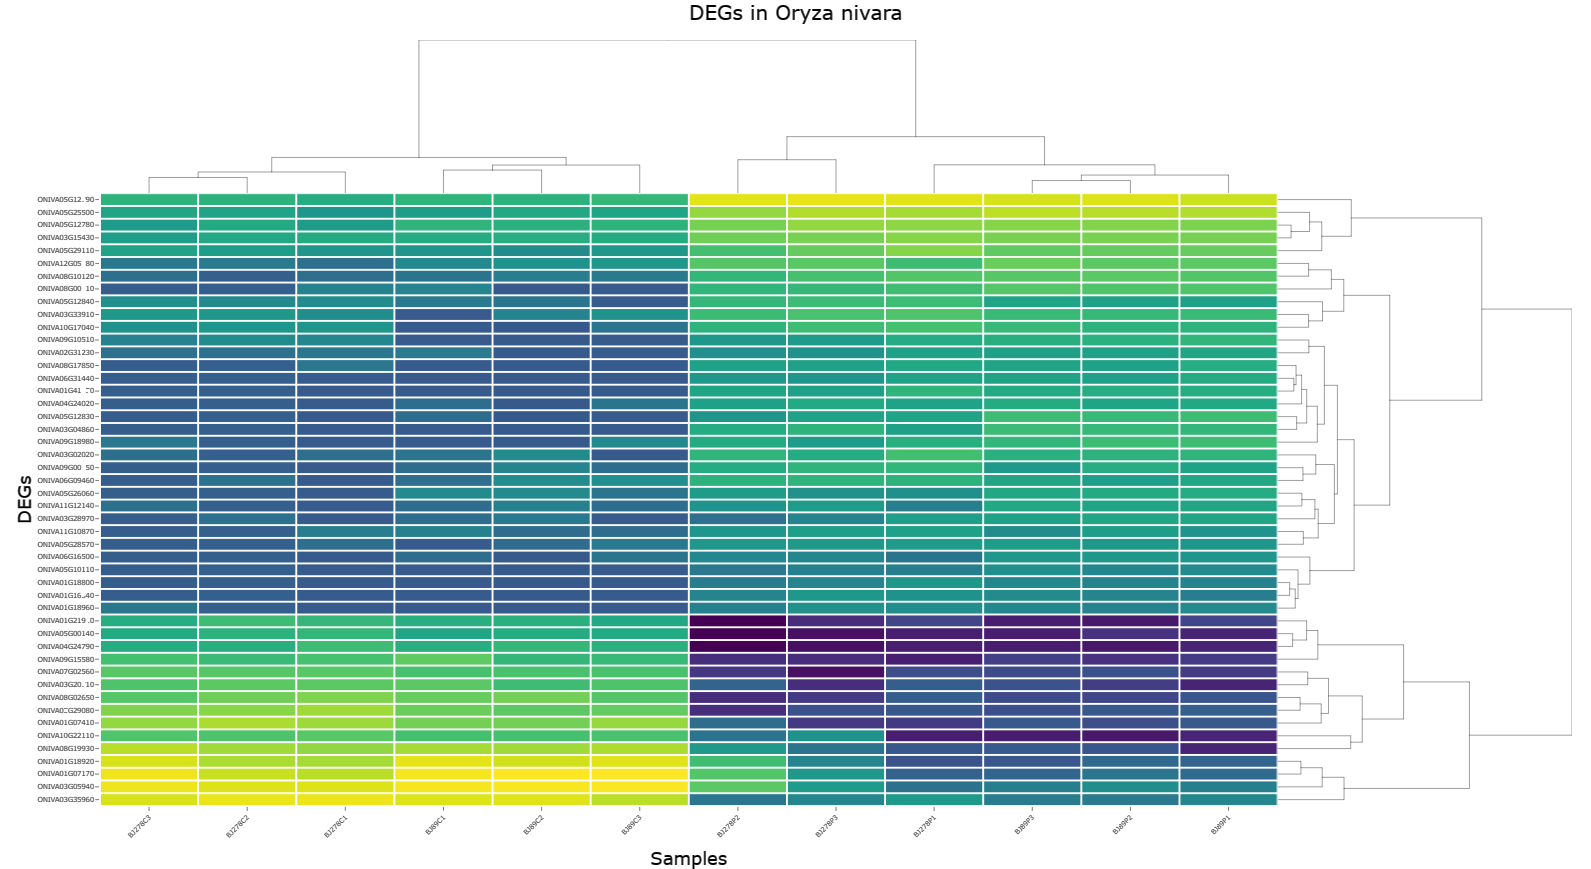
\includegraphics[width=\textwidth]{../../results/plots-and-tables/4.4-DEG-Heatmap-Oryza_nivara}
\end{figure}

\begin{figure}[htbp]
    \caption{Heatmap of the DEGs - O. sativa}
    \label{fig:4.4-DEG-Heatmap-Oryza_sativa}
    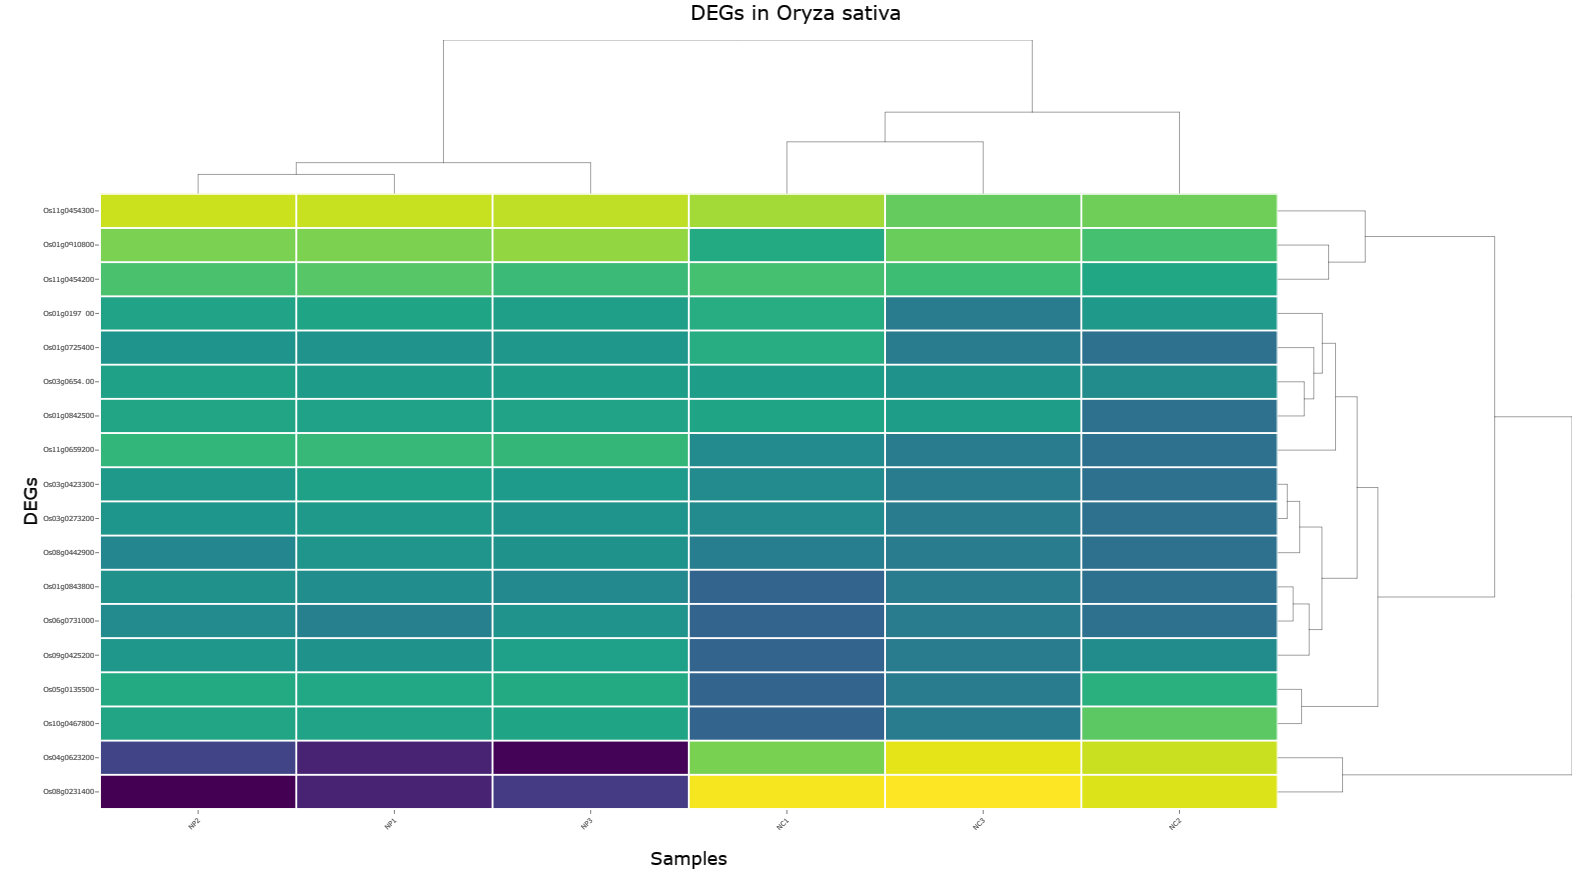
\includegraphics[width=\textwidth]{../../results/plots-and-tables/4.4-DEG-Heatmap-Oryza_sativa}
\end{figure}

\filbreak
Down- and up-regulated genes are for O. nivara:\\
{\scriptsize\texttt{ONIVA01G07170, ONIVA01G07410, ONIVA01G16640, ONIVA01G18800, ONIVA01G18920, ONIVA01G18960, ONIVA01G21950, ONIVA01G41350, ONIVA02G31230, ONIVA03G02020, ONIVA03G04860, ONIVA03G05940, ONIVA03G15430, ONIVA03G20710, ONIVA03G28970, ONIVA03G33910, ONIVA03G35960, ONIVA04G24020, ONIVA04G24790, ONIVA05G00140, ONIVA05G10110, ONIVA05G12780, ONIVA05G12790, ONIVA05G12830, ONIVA05G12840, ONIVA05G25500, ONIVA05G26060, ONIVA05G28570, ONIVA05G29080, ONIVA05G29110, ONIVA06G09460, ONIVA06G16500, ONIVA06G31440, ONIVA07G02560, ONIVA08G00310, ONIVA08G02650, ONIVA08G10120, ONIVA08G17850, ONIVA08G19930, ONIVA09G00350, ONIVA09G10510, ONIVA09G15580, ONIVA09G18980, ONIVA10G17040, ONIVA10G22110, ONIVA11G10870, ONIVA11G12140, ONIVA12G05380
}}

For O. sativa these genes are:\\
{\scriptsize\texttt{Os01g0197700, Os01g0725400, Os01g0842500, Os01g0843800, Os01g0910800, Os03g0273200, Os03g0423300, Os03g0654700, Os04g0623200, Os05g0135500, Os06g0731000, Os08g0231400, Os08g0442900, Os09g0425200, Os10g0467800, Os11g0454200, Os11g0454300, Os11g0659200
}}

A description and the location of all these genes can be found at \url{https://plants.ensembl.org}. For a deeper analysis of these genes and their potential biological significance, the available information appears to be insufficient.


\subsection{Functional enrichment analysis}

Finally, for the one-hundred top-ranked genes a statistical functional enrichment analysis\index{functional enrichment analysis} was performed to identify over- or under-represented information from gene ontology (GO)\index{gene ontology (GO)} terms. Figures \ref{fig:5.2-Gost-Plot-Oryza_nivara} and \ref{fig:5.2-Gost-Plot-Oryza_sativa} present the results as Manhattan plots.

For both O. nivara and O. sativa, the top ten GO terms belong to the major subontology "biological process (BP)"\index{gene ontology (GO)!biological process (BP)}. It appears that on the gene level the impact of drought stress may be best described and categorized in terms of biological processes as opposed to the molecular functions (MF)\index{gene ontology (GO)!molecular function (MF)} of the genes and as opposed to the cellular components (CC)\index{gene ontology (GO)!cellular component (CC)} in which the gene products are physically located.

Furthermore, for both rice species the following GO terms are significantly enriched (when just comparing the top ten GO terms): response to organic substance, response to water, response to acid chemical, response to salt, response to chemical, lignin catabolic process, phenylpropanoid catabolic process. This confirms the close relationship of the two species, and it also confirms that the GO terms are suitable to describe genetic responses to environmental factors.

\begin{figure}[htbp]
    \caption{Manhattan plot with the first 10 top-ranked GO terms highlighted - O. nivara}
    \label{fig:5.2-Gost-Plot-Oryza_nivara}
    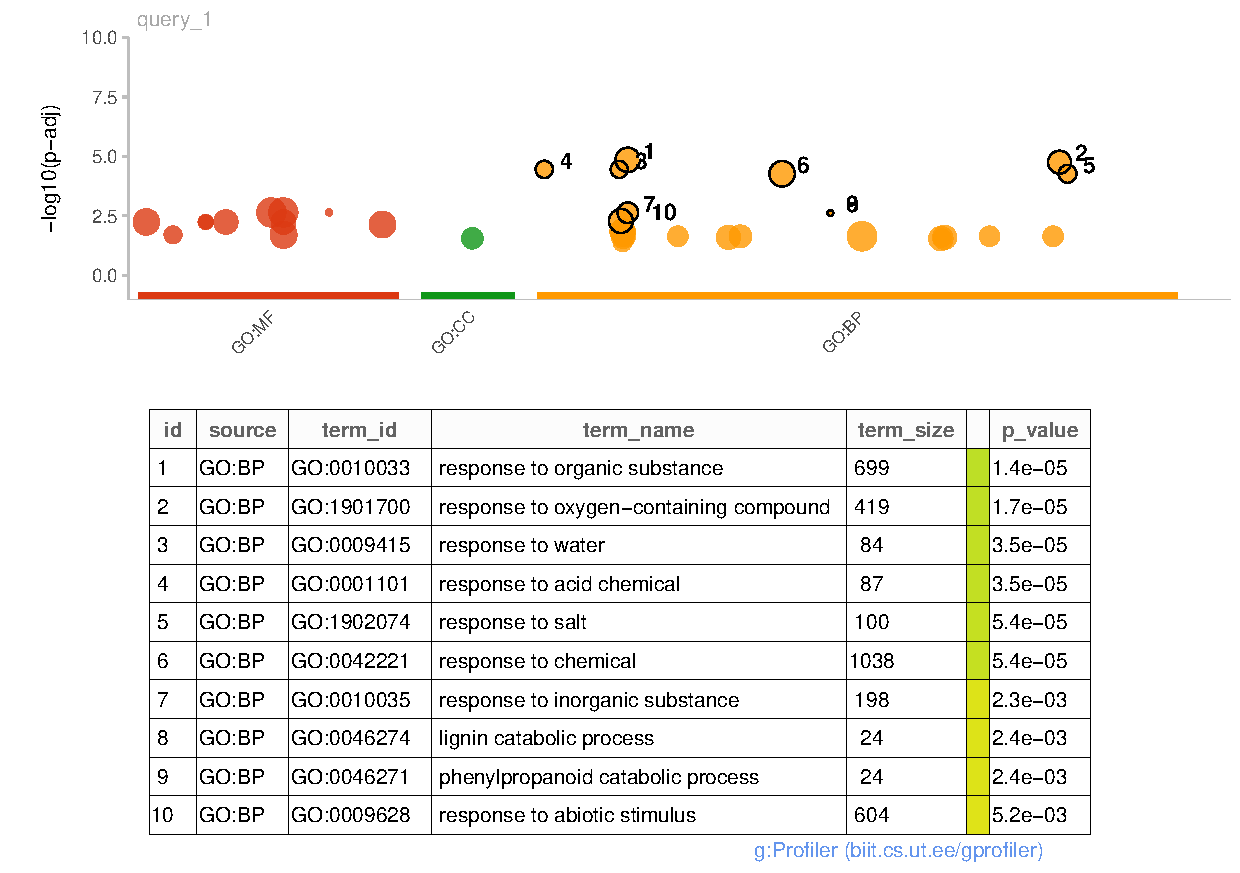
\includegraphics[width=0.9\textwidth]{../../results/plots-and-tables/5.2-Gost-Plot-Oryza_nivara}
\end{figure}

\begin{figure}[htbp]
    \caption{Manhattan plot with the first 10 top-ranked GO terms highlighted - O. sativa}
    \label{fig:5.2-Gost-Plot-Oryza_sativa}
    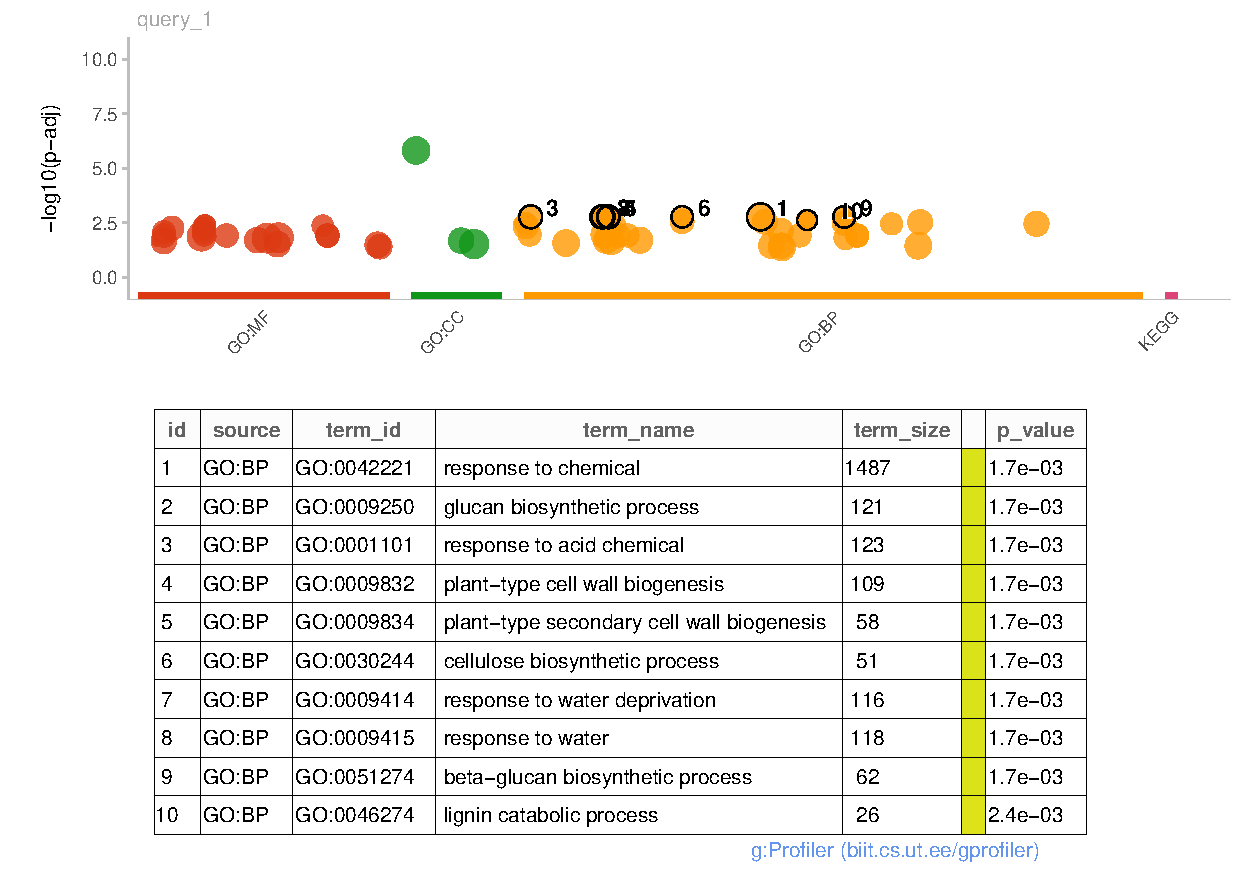
\includegraphics[width=0.9\textwidth]{../../results/plots-and-tables/5.2-Gost-Plot-Oryza_sativa}
\end{figure}